% ========================================
%	Header einbinden
% ========================================

% ==================================================
%	Festlegung der Dokumentenklasse
% ==================================================


\documentclass[paper=a4, 		% Layout für DinA4
	ngerman						% Deutsche Spracheinstellungen
	]
	{scrartcl} 					% Dokumentklasse für Aufsätze oder z.B. Praktikumsprotokolle

\usepackage{fixltx2e}			% Behebt ein paar Fehler in Latex

% ==================================================
%	Einstellen des Encodings
% ==================================================

\usepackage{ifxetex}
\usepackage{ifluatex} 

\ifxetex
	\usepackage{fontspec}
  	\usepackage{xunicode}
	\usepackage{xltxtra}
    \defaultfontfeatures{Mapping=tex-text} 	% To support LaTeX quoting style
	\setmainfont{Linux Libertine}
=======
    \defaultfontfeatures{Mapping=tex-text} % To support LaTeX quoting style
	\setmainfont{Linux Libertine} % Hier gewünschte Schriftart einfügen
\else
	\ifluatex
		\usepackage{fontspec}		% Falls das nicht funktioniert: \usepackage{luainputenc}
  		\usepackage{xunicode}
  		\defaultfontfeatures{Mapping=tex-text} % To support LaTeX quoting style
		\setmainfont{Linux Libertine} % Hier gewünschte Schriftart einfügen
	\else %pdfTeX
	  \usepackage[utf8]{inputenc}
	  \usepackage[T1]{fontenc}
	 \fi
\fi


% ==================================================
%	Spracheinstellungen
% ==================================================

\usepackage[ngerman]{babel,		% neue deutsche Rechtschreibung
	varioref}			% Bei Referenzen wird der Name des Objektes vor die Refernznummer geschrieben: z.B. \ref{bsp} liefert Seite 1

% ==================================================
%	Referenzen und Links
% ==================================================

\usepackage{hyperref}			% Verlinkungen innerhalb und außerhalb des PDF-Dokuments
\usepackage{url}			% Formattiert URLs, so dass sie sich z.B. besser vom Text abheben
\urlstyle{tt}				% TrueType-Schrift für URLs		



% ==================================================
%	Bibliograhphie
% ==================================================
%Zwei verschiedene Möglichkeiten Bibliographien einzubinden:

%	Möglichkeit 1:
% ========================
	\usepackage[numbers]{natbib}	%Paket für Bibliograhien

	%Bibtex: Nachnamen in Kapitälchen
	%\renewcommand*{\mkbibnamelast}[1]{\textsc{#1}}
	\newcommand*{\mkbibnamelast}[1]{\textsc{#1}}

	% Makros für Anhang + Referenzen
	\newcommand{\anhang}{
		\clearpage		% Anhang auf eine extra Seite packen
		\setcounter{page}{0}	
		\pagenumbering{Roman}	% Anhang wird in römischen Seitenzahlen numeriert
		\appendix		% Kapitelnummerierung in Großbuchstaben statt Zahlen.
	}

	\newcommand{\referenzen}{
		\bibliographystyle{alphadin} 			% Alphabetisch sortiert im DIN-Format
		\addcontentsline{toc}{section}{Referenzen}
		\phantomsection					% Referenzen ins Inhaltsverzeichnis
		\renewcommand{\refname}{\section*{Referenzen}\vspace*{-1em}} % Benennt das Kapitel um
		\bibliography{../include/Bibliographie.bib} 	% Die BibTeX-Datei einbinden
	}
%Zu Verwenden mit \bibliography{BIBDATEI}
% ========================
%	Möglichkeit 2:
% ========================
	%\usepackage{csquotes}				%Wird für Biblatex benötigt
	%\usepackage[style=alphabetic]{biblatex}	%Paket für Bibliograhphien mit Biblatex
%Zu Verwenden mit \bibliography{BIBDATEI} und \printbibliography oder \printbibliography[heading=bibintoc] (falls ein Inhaltsverzeichns verwendet wird)
% ==================================================



% ==================================================
%	Grafiken, Abbildungen und Tabellen
% ==================================================

\usepackage{graphicx}                   % zum Einbinden von Grafiken
\usepackage{xcolor}			% Für die Verwendung von Farben
\usepackage[font=small,			% kleine Schrift für Bildunterschriften
	labelfont=bf			% Fettgedruckte Bildunterschriften
	]
	{caption}			% Für Bildunterschriften

\usepackage{subcaption}			% Für mehrere Objekte nebeneinander mit eigenen Bildunterschriften

\usepackage{tabularx}			% Erweiterte Befehle für Tabellen
\usepackage{booktabs}			% Für professionele Tabellen, siehe Manual
\usepackage{longtable}			% Für Tabellen, die nicht mehr auf eine Seite passen.

\usepackage{rotating}			% Zum Verdrehen von Objekten. Nur mäßig verwenden.

%\graphicspath{{figs/}{bilder/}}	% Bildverzeichnisse MUSS ÃœBERPRÃœFT WERDEN!!!

% ==================================================
%	Mathematikumgebungen und Einheiten
% ==================================================

\usepackage{amsmath}			% Paket für mathematische Umgebungen und Funktionen
\usepackage{amsfonts}			% Zusätzliche Mathematische Schriftarten
\usepackage{amssymb}			% Zusätzliche Mathematische Symbole
%\usepackage{amscd}			% Zum Setzen Kommutativer Diagramme
\usepackage{amstext}			% Textsatz in der Matheumgebung
\usepackage{upgreek}			% Aufrechte griechische Buchstaben


% Diagramme mit tikz und Gnuplot zeichnen
%	\usepackage{tikz}
%	\usepackage{tikz-qtree}
%	\usepackage{gnuplot-lua-tikz}

% ==================================================
% SIUnitX: Einheiten werden vollautomatisch gesetzt
% ==================================================
\usepackage[
    separate-uncertainty = true, 		% Stellt den Fehler separat dar: Siehe SIUnitX-Manual
    mode 			= text, 			% Stellt Einheiten (Kelvin etc.) Nichtkursiv dar
    quotient-mode	= 	fraction,		% Bruchstriche nutzen
    repeatunits           = false, 
    range-phrase          = {\,bis\,},  
]{siunitx}
\sisetup{
	per-mode = fraction, 				% Bruchstriche nutzen
	output-decimal-marker = {,}, 		% Setzt das Dezimaltrennzeichen als Komma
	multi-part-units = brackets,
	exponent-product = \cdot,
}

\addto\extrasgerman{\sisetup{locale = DE}}	% "Deutsche" Einheiten
\usepackage{cancel}				% Kürzen von Einheiten in SIUnitX ermöglichen


% ==================================================
%	Sonstiges
% ==================================================

%\usepackage[official]{eurosym}			% offizielles Eurosymbol

% ==================================================
%	Seitenlayout
% ==================================================

% Kein Einrücken der Absätze (Einrücken = Null)
	\setlength{\parindent}{0pt}             % kein Einrücken der ersten Zeile in einem neuen Absatz

% Vermeidung von "Schusterjungen"
	\clubpenalty = 3000			% Höchstwert 10000, dann dürfen theoretisch keine Schusterjungen mehr auftreten.
% Vermeidkung von "Hurenkindern"
	\widowpenalty = 3000			% Höchstwert 10000, dann dürfen theoretisch keine Hurenkinder mehr auftreten.
	\displaywidowpenalty = 3000		% Es werden beide Einstellungen benötigt.

% Seitenlayout ändern mit Fancy
	\usepackage{fancyhdr}			% Paket zum bequemeren Verändern des Seitenlayouts

	% Tabellen ändern:
		\renewcommand{\thetable}{\arabic{section}.\arabic{table}} % figures bekommen die richtige Nummerierung: x.y
		\makeatletter \@addtoreset{table}{section} \makeatother      % nach jeder section wird neu gezählt

	% Kapitelüberschriften in der Kopfzeile:
		\renewcommand*{\sectionmark}[1]{\markboth{}{\thesection\ #1}}
		%\renewcommand*{\subsectionmark}[1]{\markboth{}{\thesubsection\ #1}}
		\renewcommand*{\subsectionmark}[1]{\markboth{}{}} % keine Unterüberschriften in der Kopfzeile
		\renewcommand{\plainheadrulewidth}{0.4pt}
	
	% Seitennummern rechts in der Kopfzeile:
		\lhead[\fancyplain{\thepage}{\thepage}]{\fancyplain{}{\rightmark}}
		\rhead[\fancyplain{}{\leftmark}]{\fancyplain{\thepage}{\thepage}}
	
	%Fußzeilen bleiben leer
		\lfoot{}
		\cfoot{}
		\rfoot{}




% ========================================
%	Angaben für das Titelblatt
% ========================================

\title{Versuch 353 - Das Relaxationsverhalten eines RC-Kreises\\				% Titel des Versuchs 
\large TU Dortmund, Fakultät Physik\\ 
\normalsize Anfänger-Praktikum}

\author{Jan Adam\\			% Name Praktikumspartner A
{\small \href{jan.adam@tu-dortmund.de}{jan.adam@tu-dortmund.de}}	% Erzeugt interaktiven einen Link
\and						% um einen weiteren Author hinzuzfügen
Dimitrios Skodras\\					% Name Praktikumspartner B
{\small \href{dimitrios.skodras@tu-dortmund.de}{dimitrios.skodras@tu-dortmund.de}}		% Erzeugt interaktiven einen Link
}
\date{23.Oktober 2012}				% Das Datum der Versuchsdurchführung

% ========================================
%	Das Dokument beginnt
% ========================================

\begin{document}

% ========================================
%	Titelblatt erzeugen
% ========================================

\maketitle					% Jetzt wird die Titelseite erzeugt
\thispagestyle{empty} 				% Weder Kopfzeile noch Fußzeile

% ========================================
%	Der Vorspann
% ========================================

%\newpage					% Wenn Verzeichnisse auf einer neuen Seite beginnen sollen
%\pagestyle{empty}				% Weder Kopf- noch Fußzeile für Verzeichnisse

\tableofcontents

%\newpage					% eine neue Seite
%\thispagestyle{empty}				% Weder Kopf- noch Fußzeile für Verzeichnisse
%\listoffigures					% Abbildungsverzeichnis

%\newpage					% eine neue Seite
%\thispagestyle{empty}				% Weder Kopf- noch Fußzeile für Verzeichnisse
%\listoftables					% Tabellenverzeichnis
\newpage					% eine neue Seite


% ========================================
%	Kapitel
% ========================================

%\section{Einleitung}				% Bei Bedarf

\section{Theorie}

Relaxation bezeichnet das Zurückkehren eines angeregten Systems in seinen Ruhezustand. Wird  beispielsweise ein stark gedämpftes Pendel ausgelenkt, so entsteht eine Rückstellkraft, die es wieder in seine Ruheposition zurückführt. Die asymptotische Annäherung wird durch das Relaxationsverhalten beschrieben.\\
In diesem Versuch soll ein RC-Kreis auf sein Relaxationsverhalten untersucht werden. Dieser besteht aus einem Kondensator mit der Kapazität C, der über einen Widerstand R mit einer Spannung $U_0$ auf- und entladen wird.\\
\begin{figure}[htbp]
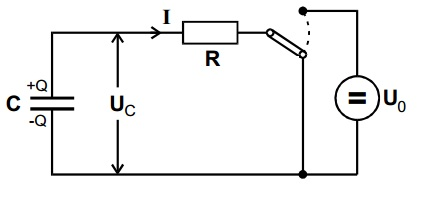
\includegraphics[width=8cm]{_pics/aufbau.jpg}
\centering
\caption{Schaltbild des Versuchs: RC-Glied wird über konstante Spannung geladen und entladen}
\end{figure}

Mit Hilfe des Kirchhoffschen und Ohmschen Gesetztes lässt sich fürs Auf- und Entladen die folgende Differentialgleichung 
für dieses System herleiten:
\begin{align}
\dot Q(t)=-\frac{1}{RC} Q(t)
\end{align}

deren Lösungen folgende Exponentialfunktionen sind:
\begin{align}
Q(t)&=Q_0(1-e^{-\frac{1}{RC}t)}\\
Q(t)&=Q_0 e^{-\frac{1}{RC}t}.
\end{align}

Der Exponent $-\frac{1}{RC}$ beschreibt dabei, wie schnell sich die Ladung des Kondensators ändert, bzw. wie schnell sich das System seinem Endzustand nähert.
RC ermöglicht es somit allgemein, qualitative Aussagen über relaxative Systeme zu treffen und wird deshalb auch als  Zeitkonstante $\tau$ des Relaxationsvorganges bezeichnet.\\

Zunächst wird das RC-Element mit einer relativ niederfrequenten ($\omega\ll\frac{1}{RC}$) Rechteckspannung $U_0$ betrieben. Die Frequenz wird so gewählt, damit sich der Kondensator bei jedem Phasendurchlauf immer noch vollständig auf- und entladen kann.
Im späteren Verlauf wird die Frequenz jedoch erhöht. Es bildet sich schließlich eine Phasenverschiebung 
\begin{align}
\varphi(\omega)=arctan(-\omega RC)
\label{varphi}
\end{align}

zwischen der Kondensatorspannung und der Generatorspannung heraus, da sich der Kondensator wegen des Widerstandes nicht instantan entladen kann.\\

Bei weiterer Erhöhung der Frequenz ist die Dauer der Phase irgendwann nicht mehr lang genug, um den Kondensator vollständig zu entladen, bzw. ihn vollständig aufzuladen.
Die Amplitude der Kondensatorspannung erreicht dann nicht mehr den Maximalwert $U_0$ und hat keinen Nulldurchlauf mehr.
Aus dem Ansatz
\begin{align*}
U_c(t)=A(\omega)cos(\omega t+\varphi\{\omega\})
\end{align*}
folgt unter Verwendung des zweiten Kirchhoffschen Gesetztes und einiger Umformungen
\begin{align}
A(\omega)= \frac{U_0}{\sqrt{1+\omega^2(RC)^2}}
\label{A_omega} .
\end{align}
Gleichung \eqref{A_omega} beschreibt die reduzierte Amplitudenhöhe in Abhängigkeit von der Frequenz $\omega$.
Das RC-Glied behindert somit den Durchfluss des Wechselstroms bei höheren Frequenzen und wird deshalb auch als Tiefpass bezeichnet, da es Ströme mit langsamen Frequenzen ungehindert durchfließen lässt, während hochfrequente Signale abgemildert werden.\\

Bei hohen Frequenzen $\omega\gg\frac{1}{RC}$ arbeitet der RC-Kreis des weiteren als Integrator. Beliebige eingegebene Signale können am Kondensator in integrierter Form abgegriffen werden, ähnlich als würde man eine Funktion integrieren.\\
Ansatz ist auch hier die Maschenregel
\begin{align*}
U(t)=U_R(t)+U_c(t)=I(t)R+U_c(t),
\end{align*}
welche umgeformt werden kann in
\begin{align*}
U(t)=RC\cdot\frac{dU_c}{dt}+U_c(t).
\end{align*}
Durch zeitliche Integration und Nährungen ergibt sich schließlich
\begin{align}
U(t)=\frac{1}{RC} \int_0^t U(t')dt'.
\label{int}
\end{align}

Gleichung \eqref{int} zeigt das Verhältnis zwischen der angelegten Wechselspannung U(t) und der am Kondensator abgegriffenen Spannung $U_c$. 
Wie man sehen kann, taucht wieder die Konstante $\frac{1}{RC}$ als charakteristische Größe auf. Diesmal ist sie der Proportionalitätsfaktor zwischen den beiden Spannungen.\\

\section{Durchführung}
\subsection{Bestimmung von RC - Methode 1}
Zunächst soll die Zeitkonstante RC bestimmt werden. Hierzu erzeugt der Generator eine Rechteckspannung mit einer hinreichend kleinen Frequenz $\omega\ll\frac{1}{RC}$, damit der Kondensator noch vollständig auf- und entladen wird und zunächst vom Wechselstrom unbeeinflusst bleibt.
Zu verschiedenen Zeitpunkten wird während der Entladung die Kondensatorspannung $U_c$ gemessen und die Daten später halblogarithmisch aufgetragen. Die Steigung der sich ergebenden Geraden entspricht der Konstanten RC.

\subsection{Bestimmung von RC - Methode 2}
Im nächsten Schritt wird der Schaltkreis mit einer Sinusspannung betrieben und die Frequenz $\omega$ schrittweise erhöht. Zu jeder Frequenz wird die Amplitude der Kondensatorspannung gemessen und alles als Graph dargestellt. Zu zeigen ist, dass bei höheren Frequenzen die Amplitude abnimmt, da die Phasendauer des Stroms zu kurz wird um den Kondensator noch vollständig aufzuladen, bzw. zu entladen. Desweiteren lässt sich mit Gleichung \eqref{A_omega} ebenfalls RC bestimmen. Die beiden Werte sollen anschließend miteinander verglichen und diskutiert werden.

\subsection{Messung der Phasenverschiebung}
Der Versuchsaufbau bleibt gleich, diesmal wird jedoch anstelle der Amplitude die Phasenverschiebung $\varphi$ zwischen der Kondensatorspannung und der Generatorspannung gemessen und überprüft, ob diese der Gleichung \eqref{varphi} genügt.

\subsection{Integrierglied}
Abschließend soll verifiziert werden, inwieweit das RC-Glied als Integrator arbeitet. Hierzu werden vom Generator nacheinander eine Sinus-, Dreieck-, und zwei verschiedene Rechteckspannungen erzeugt. 
Für die erfolgreiche Integration wird eine entsprechend hohe Frequenz gewählt und die erzeugten Graphen werden übereinander aufgetragen.

\section{Auswertung}
Hauptbetrachtungspunkt dieses Experiments ist die Bestimmung der Zeitkonstanten des bereitgestellten RC-Gliedes nach verschiedenen Methoden

\subsection{Auf- und Entladung des Kondensators}
Nach dem oben aufgeführten Schaltbild wurde das RC-Glied aufgebaut. Es wurde mit einer niederfrequenten Rechtecksspannung betrieben.
Dadurch wird der Kondensator über eine halbe Periode aufgeladen und danach entladen. Die Frequenz hierbei beträgt $f$ = 42 Hz und die Ladespannung
$U$ = 5 V. Der in der folgenden Abbildung\footnote{Bei Abbildungen vom Oszilloskop ist die x-Achse die Zeitachse mit dem als M bezeichneten Wert pro Kästchen, sowie die y-Achse die Spannungsachse mit dem als CH1/CH2 bezeichneten Wert pro Kästchen mit 0-Niveau beim an der linken Seite angebrachten Pfeil} dargestellter exponentielle Abfall entspricht der Entladekurve des Kondensators.


\begin{figure}[H]
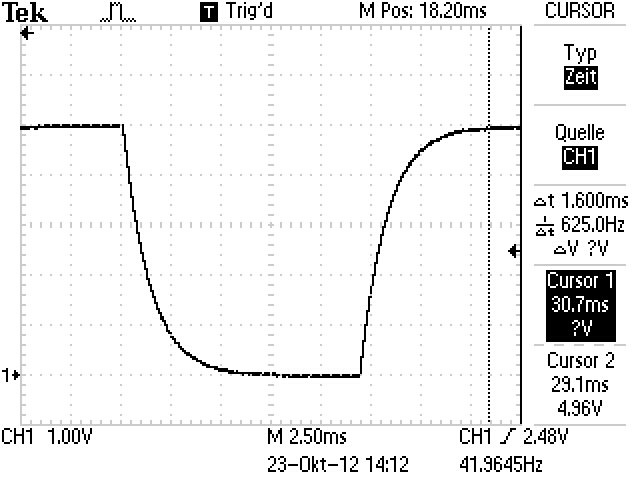
\includegraphics[width=8cm] {_pics/TEK0000.JPG}
\centering
\caption{Exponentielle Endladung des Kondensators }
\end{figure}


Um die Zeitkonstante RC zu ermitteln wird zu vielen Zeiten (x-Achse) die Spannung (y-Achse) gemessen und in halblogarithmischem Koordinatensystem
aufgeführt. Durch diese Skalierung wird der Exponent der Exponentialfunktion einer Geraden gleichgesetzt. Eine Ausgleichsgerade aus linearer 
Ausgleichsrechnung hat eine Steigung, die $\frac{1}{RC}$ enspricht. 

\renewcommand{\arraystretch}{0.8}
\begin{table}[h!]
\begin{tabular}{c|c}
$t$/ms & $U$/V\\
\hline
0,0 &	5,00\\
0,1 &	4,62\\
0,2 &	4,32\\
0,3 &	3,96\\
0,4 &	3,66\\
0,5 &	3,42\\
0,6 &	3,16\\
0,7 &	2,92\\
0,8 &	2,72\\
0,9 &	2,50\\
1,0 &	2,32\\
1,1 &	2,16\\
1,2 &	2,00\\
1,7 &	1,36\\
2,2 &	0,94\\
2,7 &	0,64\\
3,2 &	0,44\\
3,7 &	0,30\\
4,2 &	0,20\\
4,7 &	0,12\\
5,2 &	0,08\\
5,7 &	0,04 
\end{tabular}
\label{tU}
\caption{Exponentieller Abstieg der Spannung in Abhängigkeit der Zeit}
\end{table}
\renewcommand{\arraystretch}{1}

\begin{figure}[H]
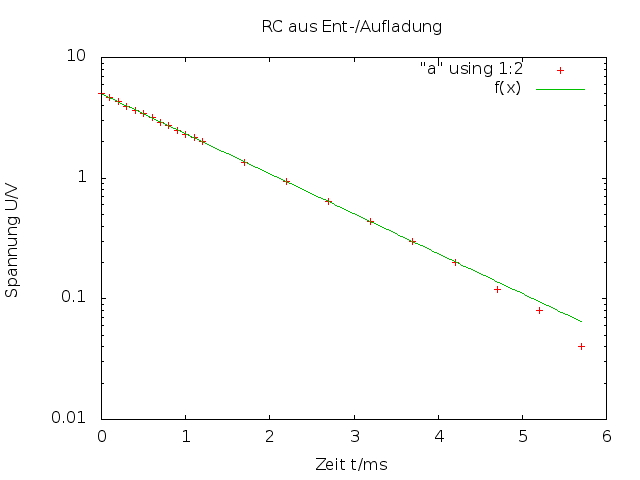
\includegraphics [width=1\textwidth] {_pics/RC1.png}
\caption{Graph zu Tabelle \eqref{tU}}
\end{figure}
\newpage

Die Steigung der Ausgleichsgeraden, durch GNUPLOT ermittelt, beläuft sich auf etwa $-7.62 \cdot 10^2$. Somit ergibt sich für die Exponentialfunktion:
\begin{align}
U(t) = U_0 \cdot \exp(-\frac{t}{RC}) \quad \text{mit} \quad RC = 1,307\cdot (1\pm 2,84 \cdot 10^{-3}) \text{ms}
\end{align}

\subsection{Frequenzabhängige Amplituden}
Indem das RC-Glied nun mit Sinusspannung höherer Frequenz betrieben wird, reicht die Periodendauer nicht aus, um 
den Kondensator komplett aufzuladen beziehungsweise zu entladen. Somit ergibt sich eine frequenzabhängige Amplitude der 
Kondensatorspannung, die entsprechend des oben aufgeführten Schaltbildes durch einen Millivoltmesser ermittelt wird. 
Die Generatorspannungsamplitude ist frequenzunabhängig bei \hspace{5cm} $U$ = 3.4 V. 

\begin{minipage}{0.2\textwidth}
\begin{tabular}{c|c}
$f$/Hz & $\frac{A(\omega)}{U_0}$\\
\hline
0 &	1\\
10 &	0.64\\
50 &	0.6\\
100 &	0.49\\
150 &	0.4\\
200 &	0.33\\
250 &	0.27\\
300 &	0.23\\
350 &	0.20\\
400 &	0.18\\
500 &	0.14\\
600 &	0.12\\
700 &	0.100\\
800 &	0.098\\
900 &	0.074\\
1000 &	0.068\\
1200 &	0.053\\
1400 &	0.044\\
1600 &	0.038\\
1800 &	0.032\\
2000 &	0.024
\end{tabular}
\end{minipage}
\begin{figure}[htbp]
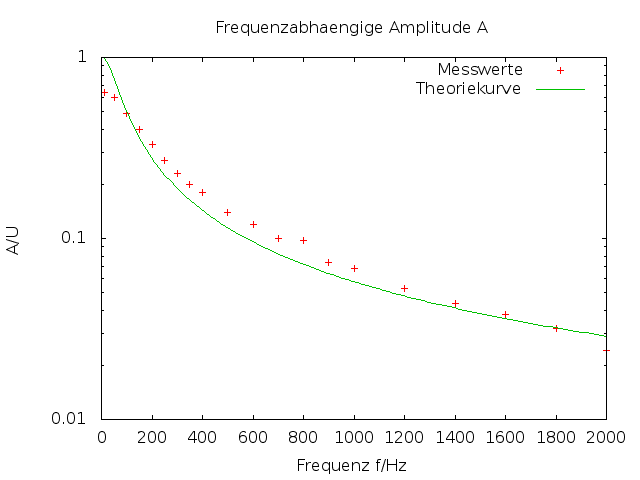
\includegraphics[width=0.8\textwidth] {_pics/RC2.png}
\centering
\caption{Die Amplitude der Kondensatorspannung in Abhängigkeit der Frequenz}
\end{figure}

Die Messwerte geben ein Verhältnis von $\frac{A(\omega)}{U}$, welches indirekt proportional zu $\omega$ ist. Die genaue
Abhängigkeit entspricht der aus Gleichung \eqref{A_omega} mit einem Wert für die Zeitkonstante, welche von GNUPLOT 
durch Ausgleichsrechnung ermittelt wird. So kann man die Formel aufführen

\begin{align}
A(\omega)= \frac{5\text{V}}{\sqrt{1+\omega^2(RC)^2}} \quad \text{mit} \quad RC = 2.76\cdot(1\pm0,116)\text{ms}
\end{align}

Dass der RC-Wert hier von dem unter 4.1 genannten abweicht, liegt an dem Innenwiderstand von $R_i = 600$ $\Omega$.

\subsection{Frequenzabhängige Phasenverschiebung}
Bei steigender Frequenz stellt sich eine Phasenverschiebung zwischen der Generatorspannung $U_0$ und der Kondensatorspannung 
$U_C$ ein. Dies läuft auf die Trägheit des RC-Gliedes hinaus, welche zunehmende Werte für $\phi$ hervorruft. Bei einem 
Zweikanal-Oszilloskop wird der Generator am ersten Eingang und das RC-Glied am zweiten Eingang verbunden, sodass die Kathodenstrahlen
beider Sinusspannungen simultan angezeigt werden können.
\begin{figure}[htbp]
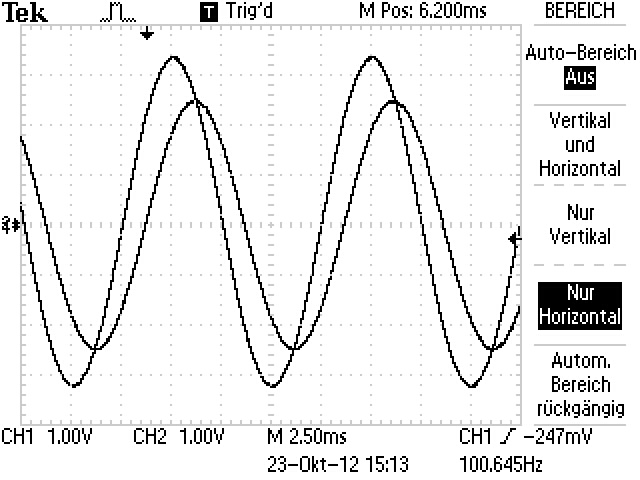
\includegraphics[width=8cm] {_pics/Phi.JPG}
\centering
\caption{Phasenverschobene Kondensator- und Sinusspannung}
\end{figure}

Nun wird die zeitliche Differenz der Nulldurchläufe a beider Schwingungen, sowie ihre Periodendauer b ermittelt und aus ihnen
$\phi$ in Abhängigkeit der Frequenz der Kondensatorspannung gemäß dem Ausdruck 

\begin{align}
 \phi = \frac{a}{b} \cdot 2 \pi 
\end{align}
bestimmt.

\begin{table}[H]
\begin{tabular}{l|r|r}
$f/Hz$ & $a/ms$	& $b/ms$\\
\hline
100 &	1.14 &	9.91\\
200 &	0.80 &	5.00\\
400 &	0.50 &	2.50\\
1000 &	0.23 &	1.00\\
2000 &	0.118 &	0.50
\end{tabular}
\caption{$a$ und $b$ in Abhängigkeit der Frequenz}
\centering
\end{table}

\begin{figure}[H]
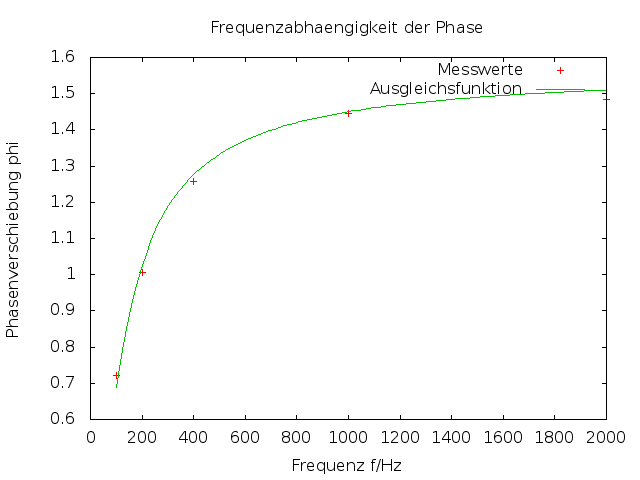
\includegraphics[width=0.7\textwidth] {_pics/RC3.png}
\centering
\label{RC3}
\caption{Arcustangensabhängigkeit zwischen der Frequenz und der Phasenverschiebung}
\end{figure}

Die von GNUPLOT gefittete Ausgleichsfunktion $f(x)$ gibt als RC-Parameter $1.311\cdot(1\pm0,036)$ms aus. $\phi$ ist proportional 
zum arcustangens von $\omega$. Für große Werte von $\omega$ beeinflusst die Zeitkonstante das Ergebnis unerheblich und der 
arcustangens nähert sich $\frac{\pi}{2}$ an, wie in Abbildung \eqref{RC3} abzusehen ist.

\subsection{RC-Glied als Integrator}
Bei gleichbleibender Schaltung soll nun mit dem Oszilloskop die Integrierfunktion des RC-Gliedes gezeigt werden. 
Hierzu werden vier verschiedene Spannungstypen angelegt und mit der Ausgabe des Kondensators verglichen. An den
Beispielen ist die Funktionsfähigkeit deutlich erkennbar.

\begin{figure}[H]
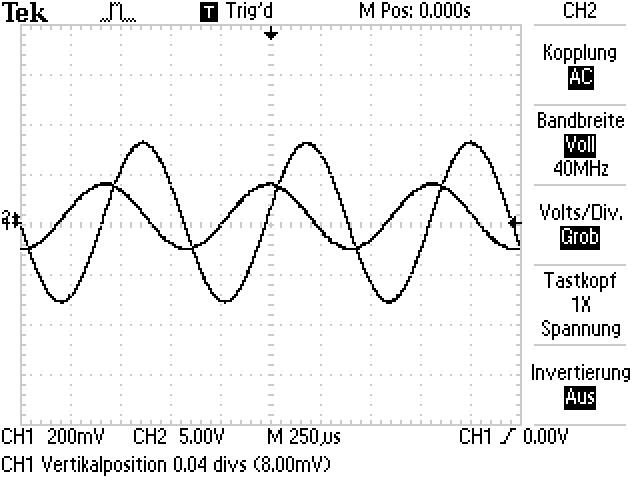
\includegraphics[height=0.4\textheight] {_pics/sinus.JPG}
\centering
\caption{Sinus zu Cosinus}
\end{figure}

\begin{figure}[H]
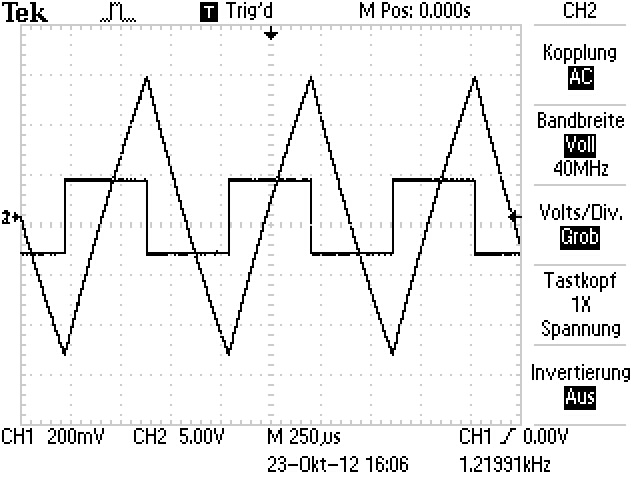
\includegraphics[height=0.4\textheight] {_pics/rechteck2.JPG}
\centering
\caption{Rechteck zu Dreieck 1}
\end{figure}

\begin{figure}[H]
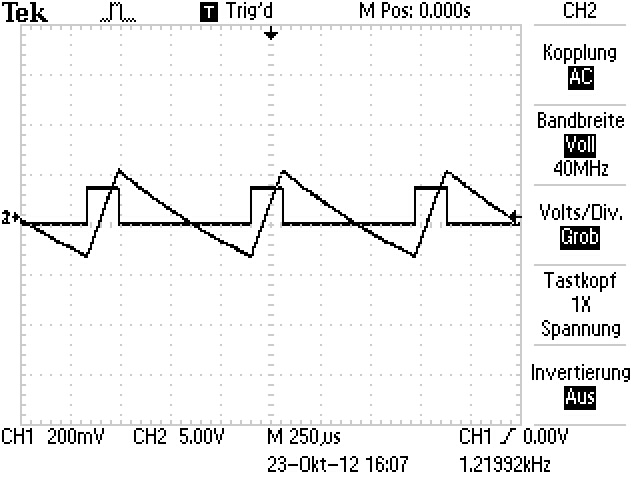
\includegraphics[height=0.4\textheight] {_pics/rechteck1.JPG}
\centering
\caption {Rechteck zu Dreieck 2}
\end{figure}

\begin{figure}[H]
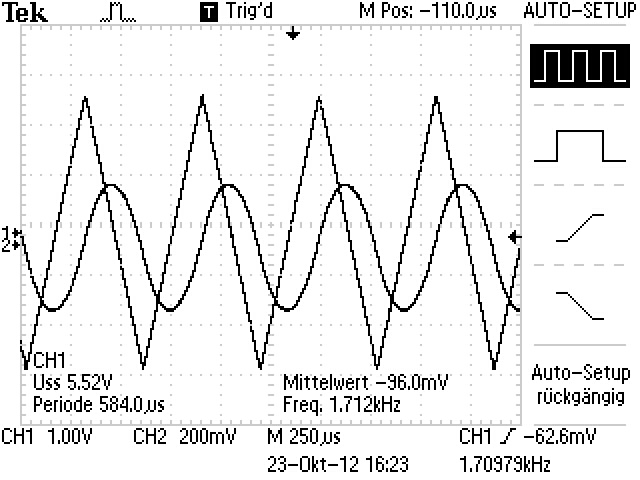
\includegraphics[height=0.4\textheight] {_pics/dreieck.JPG}
\centering
\caption {Dreieck zu Parabelbögen}
\end{figure}



% ========================================
%	Literaturverzeichnis
% ========================================

%\bibliographystyle{plainnat}			% Bibliographie-Style auswählen
%\bibliography{BIBDATEI}			% Literaturverzeichnis

% ========================================
%	Das Dokument endent
% ========================================

\end{document}